\section{Deferred proofs, construction details, and scope}
\label{app:deferred}
% =====================================================================

\subsection{Failure diagnosis}
\label{app:diagnosis}

\begin{proposition}[Dead knob, following Caveat~1 of \citet{kolchinsky2019caveats}]
\label{prop:dead}
Assume $Y = f(X)$. For every $\gamma > 0$, the CEB objective
$L_\gamma(Z) := I(X;Z|Y) - \gamma I(Y;Z)$ is minimized exactly on the corner family
$\{Z : I(Y;Z) = H(Y),\; I(X;Z|Y) = 0\}$, and the map
$\gamma \mapsto \bigl(I(X;Z^*|Y),\, I(Y;Z^*)\bigr)$ is constant. Consequently no
interior point of the IB curve is ever a Lagrangian minimizer of CEB, over the entire
parameter range.
\end{proposition}

\begin{proof}[Proof sketch (see \citet{kolchinsky2019caveats} for the full argument)]
By the chain rule, $L_\gamma(Z) = I(X;Z) - (1+\gamma)I(Y;Z)$; the data-processing
inequality gives $L_\gamma \ge -\gamma H(Y)$, attained exactly at the corner
$Z = Y$. In the Caveats paper's maximizing convention this is their Eq.~7 with
$\beta' = 1/(1+\gamma) \in (0,1)$, the range in which every maximizer is pinned at the
copy corner.
\end{proof}

The corner is a single point of the information plane and an entire equivalence class
of representations; the objective is exactly indifferent within the class, and neither
the objective nor the certificate records which member the optimizer reaches. In the
deterministic scenario this corner \emph{is} the MNI point, so CEB's declared target
and the degenerate attractor coincide. The Caveats paper repairs this by squaring the
compression term; our anchored reference supplies the same strict convexity by a
different mechanism, without squaring: a quadratic displacement term built into the
KL by construction (Proposition~\ref{prop:opb-sweep} below). We present this as a
mechanism connection to the Caveats fix, not as a new solution of the deterministic
degeneration.

\begin{proof}[Proof of Proposition~\ref{prop:geom-blind}]
For any matched pair ($b = q(z|y)$), the gap identity of Eq.~\eqref{eq:gap} gives
Eq.~\eqref{eq:reix-residual}; the matching condition is stated per class and no term
of the certificate couples two distinct class priors, so the certificate value carries
no information about the pairwise geometry of $\{q(z|y)\}$. Note that
$I(X;Z|Y)$ is generally non-zero; it vanishes only under the conditional independence
$Z \perp X \mid Y$, a property of the encoder, not of the prior.
\end{proof}

\begin{proposition}[Retention blindness on $T_\alpha$]
\label{prop:flat}
On the manifold $T_\alpha = B_\alpha \cdot Y$ of \citet{kolchinsky2019caveats}
(their Eq.~6), a family that depends on $Y$ alone, $I(X;T_\alpha|Y) = 0$ for
every $\alpha$, and with the optimal backward encoder and classifier,
$\mathrm{ReX}(T_\alpha) = 0$ and
$\CE(T_\alpha) = H(Y) - I(Y;T_\alpha) =: \delta_\alpha$: the certificate reads $0$
from the total collapse ($\alpha = 0$) to the full copy ($\alpha = 1$), while the
retained label information $I(Y;T_\alpha)$ sweeps the whole axis. Tightness of the
certificate is therefore compatible with retaining all, part, or none of $Y$: the
certificate records nothing about how much label information the code retains.
\end{proposition}

\begin{proof}
$T_\alpha$ is a function of $Y$ alone, hence $T_\alpha \perp X \mid Y$ and
$I(X;T_\alpha|Y) = 0$. By Proposition~\ref{prop:geom-blind} with the true backward
encoder the certificate is tight, $\mathrm{ReX} = I(X;T_\alpha|Y) = 0$, and the optimal
classifier attains $\langle \log c(y|z)\rangle = -H(Y|T_\alpha)$, i.e.\
$\CE = H(Y|T_\alpha) = \delta_\alpha$.
\end{proof}

\begin{remark}[The objective on $T_\alpha$ is $\beta$-independent and strictly prefers the full copy]
\label{rem:flatness}
On $T_\alpha$ the compression term contributes nothing ($\mathrm{ReX} \equiv 0$), so
the objective reads $L = \CE + \beta\,\mathrm{ReX} = \delta_\alpha$, independent of
$\beta$ and strictly minimized at $\alpha = 1$ (the full copy). No certified residual
is produced anywhere on the manifold; the blindness is that the certificate cannot
tell the optimizer --- or the analyst --- where on the retention axis the code sits.
\end{remark}

\emph{Scope of the comparison argument.} Theorem~\ref{prop:pgib-alignment} applies to
arbitrary $P_{XY}$ and every feasible comparator in the fitted model class; it does not
require $q(z|x)=p_\theta(z|y)$. Its usefulness depends on the comparator KL. Label
ambiguity, limited encoder capacity, and covariance misspecification produce the
non-zero floor made explicit in Proposition~\ref{prop:pgib-ambiguity-decomposition}.
The stronger statement that this floor is zero still requires the assumptions of
Corollary~\ref{cor:pgib-exact-alignment}: deterministic labels, exact posterior--prior
matching, and a compatible head. We do not assume those exact-realizability premises
for the real-data benchmarks. Their performance comparison evaluates utility, while
their structural diagnostics report realized mismatch and geometry. The controlled
known-noise experiment instead evaluates the ambiguity term where its population value
is analytic, including the deterministic distribution as its zero-floor special case.

\subsection{Proofs of the alignment guarantees}

\begin{proof}[Proof of Proposition~\ref{prop:opb-certificate}]
For fixed $\theta$, apply the gap identity of Eq.~\eqref{eq:gap} to the conditional
distribution $p_\theta(z|y)$ and the posterior $q_\phi$.
\end{proof}

\begin{proof}[Proof of Theorem~\ref{thm:pgib-separation}]
For (a), Jensen gives $\|m_k - m_\theta(k)\| \le \sqrt{2\tau^2_{\max} D_k}$, and the
triangle inequality on
$m_i - m_j = (m_i - m_\theta(i)) + (m_\theta(i) - m_\theta(j))
+ (m_\theta(j) - m_j)$ gives Eq.~\eqref{eq:pgib-separation}. For (b), the same two
inequalities hold pointwise for $P_Y$-a.e.\ $y$: Jensen on the regular conditional
expectation gives
$\|m(y) - m_\theta(y)\| \le \sqrt{2\tau^2_{\max} D(y)}$ (the norm is convex), and
the triangle inequality gives Eq.~\eqref{eq:pgib-separation-continuous}; intersecting
the two measure-one sets of valid $y$'s yields the almost-everywhere pair statement.
\end{proof}

\begin{remark}[Finite-sample estimation of the continuous case]
\label{rem:pgib-binning}
On finite samples the regular conditional expectations of part (b) are estimated by
binning the label axis into intervals $B_i$ with representative labels $\bar y_i$
and centers $m_i = \E[\mu_\phi(X) \mid Y \in B_i]$; the bin diameter adds a
quantization error bounded by
$\rho_{\max}\,\operatorname{diam}(B_i) + \rho_{\max}\,\operatorname{diam}(B_j)$ (by
the upper bound of Eq.~\eqref{eq:pgib-lipschitz}), which vanishes as the bins
shrink. The separation statement itself is pointwise and needs no binning.
\end{remark}

\begin{proof}[Proof of Theorem~\ref{prop:pgib-alignment}]
Since $\Sigma_\theta(y)\preceq\tau^2_{\max}I_d$, the Gaussian KL contains a mean
term at least
$\|\mu_\phi(x)-m_\theta(y)\|^2/(2\tau^2_{\max})$. Hence
$\mathcal D(\widehat w)\le\mathcal K(\widehat w)$. For any feasible $w_0$,
near-optimality and non-negativity of the prediction loss give
\begin{equation*}
\beta\mathcal K(\widehat w)
\le \mathcal R(\widehat w)+\beta\mathcal K(\widehat w)
\le \mathcal R(w_0)+\beta\mathcal K(w_0)+\varepsilon.
\end{equation*}
Division by $\beta$ proves Eq.~\eqref{eq:pgib-comparator-bound}; substituting
$\mathcal K(w_0)\le\delta_{\mathrm{app}}$ and
$\mathcal R(w_0)\le C_{\mathrm{app}}$ proves
Eq.~\eqref{eq:pgib-approximate-alignment}.
\end{proof}

\begin{proof}[Proof of Proposition~\ref{prop:pgib-ambiguity-decomposition}]
For OPB let $A_Y:=a q_{0,Y}$. Conditional on $X$, orthonormality gives
$\E[A_Y\mid X]=a\sum_k\eta_k(X)q_{0,k}$ and
\begin{equation*}
\E\!\left[\|A_Y-\E[A_Y\mid X]\|^2\mid X\right]
=a^2\left(1-\|\eta(X)\|_2^2\right).
\end{equation*}
The conditional bias--variance identity then yields
\begin{equation*}
\E\|h(X)-A_Y\|^2
=a^2\E[1-\|\eta(X)\|_2^2]
+\E\left\|h(X)-a\sum_k\eta_k(X)q_{0,k}\right\|^2.
\end{equation*}
Adding the diagonal-Gaussian covariance term $V_0$ proves
Eq.~\eqref{eq:opb-ambiguity-decomposition}. For EPB set
$A_Y:=\rho\tilde Y u_0$. Then
$\E[A_Y\mid X]=\rho\nu(X)u_0$ and
$\E[\|A_Y-\E[A_Y\mid X]\|^2\mid X]
=\rho^2\operatorname{Var}(\tilde Y\mid X)$. The same identity plus $V_0$ proves
Eq.~\eqref{eq:epb-ambiguity-decomposition}.
\end{proof}

\begin{proof}[Proof of Corollary~\ref{cor:pgib-exact-alignment}]
For classification, the assumed comparator $q(z|x)=p_\theta(z|y)$ has
$\mathcal K(w_0)=0$. Its Bayes cross-entropy is
$C_{\mathrm G}=H(Y\mid Z_{\mathrm{align}})\le\ln K$; with shared covariance the
determinant factors cancel and its posterior is the anchor-energy rule. Applying
Eq.~\eqref{eq:pgib-comparator-bound} gives Eq.~\eqref{eq:pgib-alignment}. For
regression the aligned comparator again has zero KL. Under the tied head its error is
$(\tau/\rho)\eta$, $\eta\sim\mathcal N(0,1)$, so its standardized squared risk is
$\tau^2/\rho^2$; the same theorem gives
Eq.~\eqref{eq:pgib-alignment-regression}.
\end{proof}

\begin{proof}[Proof of Corollary~\ref{cor:pgib-alignment-separation}]
Theorem~\ref{prop:pgib-alignment} gives $\E[D(Y)]\le B_0$.
For (a), $D_k\le B_0/\pi_k$; substituting this into
Theorem~\ref{thm:pgib-separation}(a) gives
Eq.~\eqref{eq:pgib-alignment-separation}. For (b), Markov's inequality gives
$P_Y(D(Y)>t)\le B_0/t$; on $S_t$ the pointwise inequality of
Theorem~\ref{thm:pgib-separation}(b) applies with $D(y),D(y')\le t$.
\end{proof}

\begin{proof}[Proof of Proposition~\ref{prop:opb-collapse}]
By Jensen's inequality the left side is at least
$\tfrac{1}{2\tau^2}\sum_k \pi_k \|c - a q_{\theta,k}\|^2
= \tfrac{1}{2\tau^2}\bigl(\|c\|^2 - 2a\,c^{\top}\!\sum_k\pi_k q_{\theta,k} + a^2\bigr)$.
Minimizing over $c$ gives $c = a\sum_k\pi_k q_{\theta,k}$; by orthonormality
$\|\sum_k\pi_k q_{\theta,k}\|^2 = \sum_k \pi_k^2$, yielding Eq.~\eqref{eq:opb-collapse}.
\end{proof}

\begin{remark}[What the framework constrains (and what it does not)]
\label{rem:counterexample}
The constraints of the geometric prior bind the reference, not the deployed
representation: for any orthonormal frame $\{q'_k\}$ and the class-constant posterior
$q(z|Y=k) = \mathcal{N}(a\,q'_k, \tau^2 I_d)$, the trainable frame can rotate
to match ($q_{\theta,k} \to q'_k$), yielding $\KL = 0$, $I(X;Z|Y) = 0$, and
$I(Y;Z) > 0$: a full-retention label code with a zero certificate. The framework
therefore constrains the geometric \emph{form} of the label code (precisely what CEB
left unspecified), and does not claim that the certificate meters retained label
information. In the fixed-covariance canonical instance, the remaining freedom at
certificate zero is the frame rotation. The covariance-relaxed real-data protocol has
an additional but log-clamped matching channel; the comparison theorem applies with
the resulting $\tau^2_{\max}$, and Section~\ref{sec:direct-mismatch} reports that
channel rather than treating it as fixed.
\end{remark}

\subsection{Construction details}
\label{app:construction}

\begin{assumption}[Full rank]
\label{ass:fullrank}
$U_\theta$ has full column rank wherever the polar factor and its backward pass are
evaluated; this is monitored rather than imposed by an extra loss.
\end{assumption}

\paragraph{Polar permutation equivariance.} For any label permutation matrix $P$,
\begin{equation}
Q_\theta(U_\theta P)
= U_\theta P \bigl( P^{\top} U_\theta^{\top} U_\theta P \bigr)^{-1/2}
= U_\theta \bigl( U_\theta^{\top} U_\theta \bigr)^{-1/2} P
= Q_\theta(U_\theta)\, P ,
\label{eq:opb-equivariance}
\end{equation}
since $P P^{\top} = I_K$ and the inverse square root conjugates under $P$. Permuting
the label numbering therefore permutes the anchors accordingly, and no class index
plays a distinguished role.

\begin{proposition}[Orthogonal class-prior geometry by construction]
\label{prop:opb-frame}
Under Eqs.~\eqref{eq:opb-qr}--\eqref{eq:opb-prior}, the class means
$a_k = a\,q_{\theta,k}$ satisfy Eq.~\eqref{eq:opb-geometry}; equivalently, the
class-mean Gram matrix is $a^2 I_K$: under Assumption~\ref{ass:fullrank}, the prior
supplies a class-separated spherical code at every training step, whatever the
optimizer does.
\end{proposition}

\begin{proof}
Eq.~\eqref{eq:opb-geometry} follows from $Q_\theta^{\top}Q_\theta = I_K$ after scaling
by $a$; in particular
$\|a_i - a_j\|^2 = \|a_i\|^2 + \|a_j\|^2 - 2a_i^{\top}a_j = 2a^2$.
\end{proof}

\begin{proposition}[Anchor-energy classifier equivalence]
\label{prop:opb-energy}
The scores $s_k(z)=-\|z-aq_{\theta,k}\|^2/(2\tau^2)+\log\pi_k$ are Gaussian Bayes
scores up to a class-independent term. For uniform classes, the corresponding linear
weights are $(a/\tau^2)q_{\theta,k}$.
\end{proposition}

\paragraph{Initialization, monitoring, and re-initialization.} The posterior logvar
head is zero-initialized ($\sigma^2 = \tau^2 = 1$ at initialization, so training
starts at $\KL \approx \tfrac{1}{2\tau^2} a^2$); the prior encoder is
identity-initialized, so the initial raw matrix is $U_\theta = [e_1, \dots, e_K]$,
full column rank, with a stable polar-factor backward (the verified condition of
Assumption~\ref{ass:fullrank}). The full-rank condition is \emph{verified, not
imposed}: $\sigma_{\min}(U_\theta)$ is monitored along training and stays bounded
away from zero in the reported runs, and no additional regularizer is added to the
objective, which remains Eq.~\eqref{eq:opb-objective} exactly. Near rank deficiency
the polar factor's gradient is delicate; should the monitor flag a near-deficient
step, the recommended handling is a re-initialization of the prior encoder (the
reported runs never triggered it).

\paragraph{Covariance protocol.} Equations~\eqref{eq:opb-prior} and
\eqref{eq:epb-prior} define the fixed-covariance canonical instances used for the
exact Bayes-head equivalence and the controlled label-ambiguity experiment of
Section~\ref{sec:controlled-validation}. The real-data benchmark protocol retains the
common CEB parameterization of a learned label-conditional diagonal covariance, with
log-variance clamped to a fixed interval. It is therefore a covariance-relaxed member
of $\mathcal G$: the OPB/EPB mean geometry and readout scale remain fixed, while
Eq.~\eqref{eq:pgib-covariance} holds with the clamp-induced $\tau^2_{\max}$.
Proposition~\ref{prop:opb-energy} is an exact Gaussian Bayes equivalence only for the
shared-covariance canonical instance; in the relaxed benchmark it remains a
zero-parameter readout of the same anchor means. The direct diagnostics in
Section~\ref{sec:direct-mismatch} use each checkpoint's realized conditional
covariance rather than silently substituting the canonical $\tau^2I$.

\paragraph{EPB axis choices.} Three variants of the direction: (A) \emph{fixed
axis}, $u = [1, 0, \dots, 0]$, with no trainable prior direction: the
theoretically cleanest ablation, at the price of prespecifying a latent coordinate;
(B) \emph{trainable normalized axis}, $u = W/\|W\|$ with $W$ trained and normalized
at every step, our main variant, which keeps the scale $\rho$ exact while allowing
the model to choose the axis; (C) \emph{unconstrained linear axis},
$\mu_p(y) = W \tilde y$: the simplest ablation, still isometric by linearity but
with a free scale that can shrink and weaken the geometry. We recommend (B), use (A)
to test whether the trainable rotation carries the benefit, and keep (C) as a
diagnostic. The main variant uses no bias: an affine offset cancels in pairwise
distances but is a free extra degree of matching, and $\tilde y$ is already centered.

\paragraph{EPB isometry notes.} The isometry is exact and global: any nonzero linear
map of a scalar label is isometric up to its norm, and the normalization fixes that
norm to $\rho$; unlike fixed random-feature anchors, whose pairwise distances grow
nonlinearly and saturate, the isometric axis preserves label distances at every scale
(with the price that anchor norms grow with $|\tilde y|$; a line and a fixed-radius
sphere intersect in at most two points, so isometry and equal norms cannot both hold).
All prior means lie on one line; for $y_i < y_j < y_k$ the distances add,
$\|\mu_p(y_i)-\mu_p(y_k)\| = \|\mu_p(y_i)-\mu_p(y_j)\| + \|\mu_p(y_j)-\mu_p(y_k)\|$:
order and magnitude of label differences are encoded exactly.

\paragraph{Multidimensional regression labels.} For $y \in \R^m$ ($m \le d$), the
same construction extends verbatim: take $W \in \R^{d \times m}$, its thin polar
factor $Q = W (W^{\top}W)^{-1/2}$, and the prior $\mu_p(y) = \rho\, Q\, \tilde y$,
which is isometric in the label metric; the scalar case is $m = 1$ with $Q = u$. The
label metric must be declared before standardization, otherwise ``isometric'' has no
unique meaning.

\subsection{Additional results}

\begin{lemma}[OPB KL decomposition]
\label{lem:opb-kl-decomposition}
For a diagonal posterior covariance and the prior of Eq.~\eqref{eq:opb-prior},
\begin{equation}
\KL\bigl(q_\phi(z|x)\,\|\,p_\theta^{\mathrm{OPB}}(z|y)\bigr)
= \frac{1}{2\tau^2}\|\mu_\phi(x) - a\,q_{\theta,y}\|^2
+ \frac12 \sum_{r=1}^{d}\Bigl[
\frac{\sigma_{\phi,r}^2(x)}{\tau^2} - 1 - \log\frac{\sigma_{\phi,r}^2(x)}{\tau^2}
\Bigr],
\label{eq:opb-kl-decomposition}
\end{equation}
a class-anchor mismatch term plus a variance mismatch term that is non-negative and
vanishes exactly at $\sigma_{\phi,r}^2(x) = \tau^2$ for all $r$. The mismatch term is
quadratic in the displacement to a reference whose scale and covariance cannot move:
this is the mechanism behind the strict convexity of
Proposition~\ref{prop:opb-sweep} below.
\end{lemma}

\begin{proof}
Apply the diagonal-Gaussian KL formula with posterior mean $\mu_\phi(x)$, prior mean
$a\,q_{\theta,y}$, posterior variances $\sigma_{\phi,r}^2(x)$, and the fixed prior
variance $\tau^2$.
\end{proof}

\begin{corollary}[Label-information lower bound in the aligned Gaussian model]
\label{cor:opb-fano}
Assume uniform classes and exact alignment
$q(z|Y=k) = \mathcal{N}(a\,q_{\theta,k}, \tau^2 I_d)$. The pairwise error probability
of the nearest-anchor classifier is
$P_{\mathrm{pair}} = \Phi\bigl(-\frac{a}{\sqrt{2}\,\tau}\bigr)$, with
$P_e \le \min\{1, (K-1)P_{\mathrm{pair}}\}$, and whenever the displayed bound
$\bar P_e \le 1 - 1/K$, Fano's inequality gives
$I(Y;Z) \ge \log K - h_2(\bar P_e) - \bar P_e \log(K-1)$. This links the anchor
scale-to-noise ratio $a/\tau$ to the retained label information, conditionally on the
aligned Gaussian model.
\end{corollary}

\begin{proof}
Two anchors have distance $\sqrt{2}a$ by Proposition~\ref{prop:opb-frame}; the
equal-covariance binary decision boundary is halfway between them, giving
$\Phi(-\sqrt{2}a/(2\tau))$. The union bound and Fano's inequality on
$[0, 1-1/K]$ conclude.
\end{proof}

\begin{proposition}[Joint strict convexity and unique optimum on a restricted aligned surrogate]
\label{prop:opb-sweep}
Consider the class-symmetric aligned family: every input of class $y$ is mapped to the
posterior $q_y = \mathcal{N}(s\,q_{\theta,y}, \sigma^2 I)$ ($s \ge 0$, $\sigma^2 > 0$;
anchor scale $a > 0$), and the classifier is the anchor-energy classifier of
Proposition~\ref{prop:opb-energy} (weights $w_j = c\,q_{\theta,j}$ with scale
$c = a/\tau^2$ fixed by construction). With the \emph{stochastic training code}
$z \sim q_y$ (as in the actual objective, Eq.~\eqref{eq:opb-objective}), the
training cross-entropy is
\begin{equation}
g(s, \sigma^2) := \E_\eta\Bigl[
\ln\Bigl(1 + \textstyle\sum_{j \ne y} e^{-cs + c\sigma(\eta_j - \eta_y)}\Bigr)
\Bigr],
\qquad \eta \sim \mathcal{N}(0, I_K),
\label{eq:opb-ce-train}
\end{equation}
and the training Lagrangian is
\begin{equation}
L_\beta(s, \sigma^2) = g(s, \sigma^2)
+ \beta\Bigl[
\tfrac{1}{2\tau^2}(s-a)^2
+ \tfrac{d}{2}\bigl(\sigma^2/\tau^2 - 1 - \ln(\sigma^2/\tau^2)\bigr)
\Bigr].
\label{eq:opb-lag-train}
\end{equation}
Then for every $\beta > 0$, $L_\beta$ is strictly convex jointly in $(s, \sigma)$ and
has a unique joint minimizer $(s^*(\beta), \sigma^*(\beta))$, interior in $s$ since
$a > 0$: the stochastic training objective has a well-defined optimum, in contrast to
the deterministic IB Lagrangian, whose optimum is pinned at a corner for every $\beta$
(Proposition~\ref{prop:dead}). This is a \emph{restricted surrogate result}: it
analyzes two scalar variables on the class-symmetric aligned family, with the frame,
the anchor scale, and the classifier scale held fixed; the full OPB objective, with
its nonlinear posterior, trainable frame, and non-convex degrees of freedom, lies
outside this analysis, and the result neither establishes $\beta$-tunability of the
full objective nor makes any claim on the information plane.
The deterministic evaluation code ($z = \mu$) is the $\sigma \to 0$ limit, and
$g \ge \ln(1 + (K-1)e^{-cs})$ by Jensen (the log-sum-exp is convex), so the statement
strictly generalizes the deterministic surrogate analysis. We do \emph{not} claim here
that the map $\beta \mapsto s^*(\beta)$ is monotone or that the sweep is one-to-one:
the minimizer $\sigma^*$ responds to $\beta$ through the cross-derivative
$\partial^2 g/\partial s\,\partial\sigma$, and establishing the sign of
$\mathrm{d}s^*/\mathrm{d}\beta$ requires the full two-dimensional stationarity
analysis, which we leave open; the $\beta$-sweep is reported empirically in the
experiments. The fixed-scale condition holds for the main model by construction
(Proposition~\ref{prop:opb-energy}), so the statement describes the actual training
objective up to the aligned-family idealization. We do not analyze the free-classifier
variant on this surrogate: under the stochastic training code, a diverging classifier
scale does not produce a degenerate solution: at $\operatorname{KL} \to 0$ the
posterior variance is pinned at $\sigma^2 = \tau^2 > 0$, so the class-conditional
Gaussians overlap and the training cross-entropy of a free classifier diverges with
its scale rather than vanishing (for $K = 2$ it contains
$\E[\ln(1 + e^{-c(a + \tau\xi)})]$, whose integrand grows linearly in $c$ on the
event $\xi < -a/\tau$, which has positive probability). An analysis of the free
classifier would require an explicit classifier-norm constraint or regularizer and is
left to future work.
\end{proposition}

\begin{proof}
For each fixed $\eta$, the integrand of Eq.~\eqref{eq:opb-ce-train} is a log-sum-exp of
functions affine in $(s, \sigma)$ (the constant $1$ has slope zero and each exponential
has slope $(-c,\, c(\eta_j - \eta_y))$), hence jointly convex in $(s, \sigma)$, and the
expectation $g$ is jointly convex. No strictness is claimed for $g$: for $K = 2$ the
integrand depends on $(s, \sigma)$ only through the single linear combination
$-cs + c\sigma(\eta_2 - \eta_1)$, so its Hessian has rank one. Write the KL term as
$R(s, \sigma) := \tfrac{1}{2\tau^2}(s-a)^2
+ \tfrac{d}{2}\bigl(\sigma^2/\tau^2 - 1 - \ln(\sigma^2/\tau^2)\bigr)$; its Hessian in
$(s, \sigma)$ is
$\nabla^2 R = \operatorname{diag}\bigl(\tau^{-2},\; d\,(\tau^{-2} + \sigma^{-2})\bigr)$,
strictly positive definite for every $\sigma > 0$, so $\beta R$ is strictly convex in
$(s, \sigma)$. Hence $L_\beta = g + \beta R$ is the sum of a jointly convex and a
strictly convex function, and is strictly convex in $(s, \sigma)$. Since
$R \to +\infty$ as $s \to \infty$, $\sigma \to 0^+$, or $\sigma \to \infty$, the
sublevel sets of $L_\beta$ are compact, and the unique joint minimizer exists (by
strict convexity it is unique). For $a > 0$ the minimizer is interior in $s$: at
$s = 0$, $\partial L_\beta/\partial s = -c\,\E[p_{\mathrm{w}}] - \beta a/\tau^2 < 0$,
where $p_{\mathrm{w}}$ is the error probability of the sampled code, so $s^* > 0$.
\end{proof}

\begin{remark}[The sweep is a KL--CE surrogate curve; scope and limitations]
\label{rem:opb-scope}
Proposition~\ref{prop:opb-sweep} proves joint strict convexity and uniqueness of the
optimum for the stochastic training objective in the KL--CE plane on the aligned family
at fixed classifier scale: a restricted surrogate result, which does not establish
$\beta$-tunability of the full OPB objective, and in any case not a statement on the
information plane of the Caveats paper; the results of the main text
establish a structured conditional prior, an exact KL geometry, and conditional
separation guarantees, and they do \emph{not} establish a mutual information upper
bound tighter than CEB's: Eq.~\eqref{eq:opb-certificate} is the usual CEB gap
identity for a particular prior family. The orthogonal-frame construction fixes all pairwise anchor
distances, so the framework should not claim to recover arbitrary semantic class
similarities. All geometric statements are conditional on
Assumption~\ref{ass:fullrank}: orthonormality holds exactly by the polar construction
wherever the factorization exists, and the condition is verified, not imposed,
along the reported runs (Section~\ref{sec:opb}); the construction is exactly
equivariant under relabeling of the classes by Eq.~\eqref{eq:opb-equivariance}, so
no class index plays a distinguished role. If the frame were computed from the
current input batch rather than from the all-class prior matrix, the prior would
become batch-dependent and Proposition~\ref{prop:opb-certificate} would no longer
follow directly. Finally, the
anchor-energy classifier of Proposition~\ref{prop:opb-energy} fixes the classifier
scale to $a/\tau^2$ by construction, removing the independent classifier-margin
escape route in the aligned surrogate of Proposition~\ref{prop:opb-sweep}; whether a
free classifier (with an explicit norm constraint or regularizer) admits its own
degenerate route is left to future work, and the free linear classifier is kept in
the experiments as a variant for comparison.
Whether the joint optimum of Proposition~\ref{prop:opb-sweep} moves monotonically in
$\beta$ is likewise open: it requires the full two-dimensional stationarity analysis,
in which the optimal variance responds to $\beta$ through the cross-derivative
$\partial^2 g/\partial s\,\partial\sigma$ of the stochastic cross-entropy.
The trainable frame and axis constitute a rotation channel that this paper does not
address: the certificate's zero set contains the full-retention orthogonal label codes
at any frame rotation (the reference can rotate to meet them), and the framework pins
the \emph{geometry of the code}; it does not claim that the certificate reads off
the retained label information. Quantifying how much of the anchor gap is absorbed by
frame rotation rather than by posterior motion is left to future work (a frozen-frame
ablation isolates it).
\end{remark}

\subsection{Controlled label-ambiguity sensitivity analyses}
\label{app:noisy-alignment-sensitivity}

Training evaluates the population objective by weighting all $K^2$
clean/observed-label pairs by the noise model, with a descending-$\beta$ warm start
to remove avoidable optimization error at the small-$\beta$ end; the comparator risk
$C_{\rm comp}(r)$ is estimated by Monte Carlo. The population-weighted experiment of
Section~\ref{sec:controlled-validation} uses a fixed frame and the standard trainable
posterior variance. Figure~\ref{fig:noisy-alignment-sensitivity} changes these
choices one at a time. Fixing the posterior variance to
$\sigma^2\equiv\tau^2$ leaves the measured mismatch on the analytic floors, confirming
that the result is not produced by a covariance compensation channel. Replacing the
fixed frame by the trainable stateless polar frame gives the same result, so the floor
is invariant to the learned rigid frame rotation.

The third panel replaces the exact population weights by sampled noisy labels. It
shows the expected finite-sample displacement from the population floor at weak
compression and convergence toward the empirical floor as compression strengthens.
Six sampled-label configurations at large $\beta$ fail the explicit comparator-objective
gate (twelve stored rows because both best and final checkpoints are retained); they are
marked as optimization failures rather than interpreted as violations of
Eq.~\eqref{eq:pgib-comparator-bound}. The population-weighted main grid and both
structural controls satisfy the gate at every point.

\begin{figure*}[t]
\centering
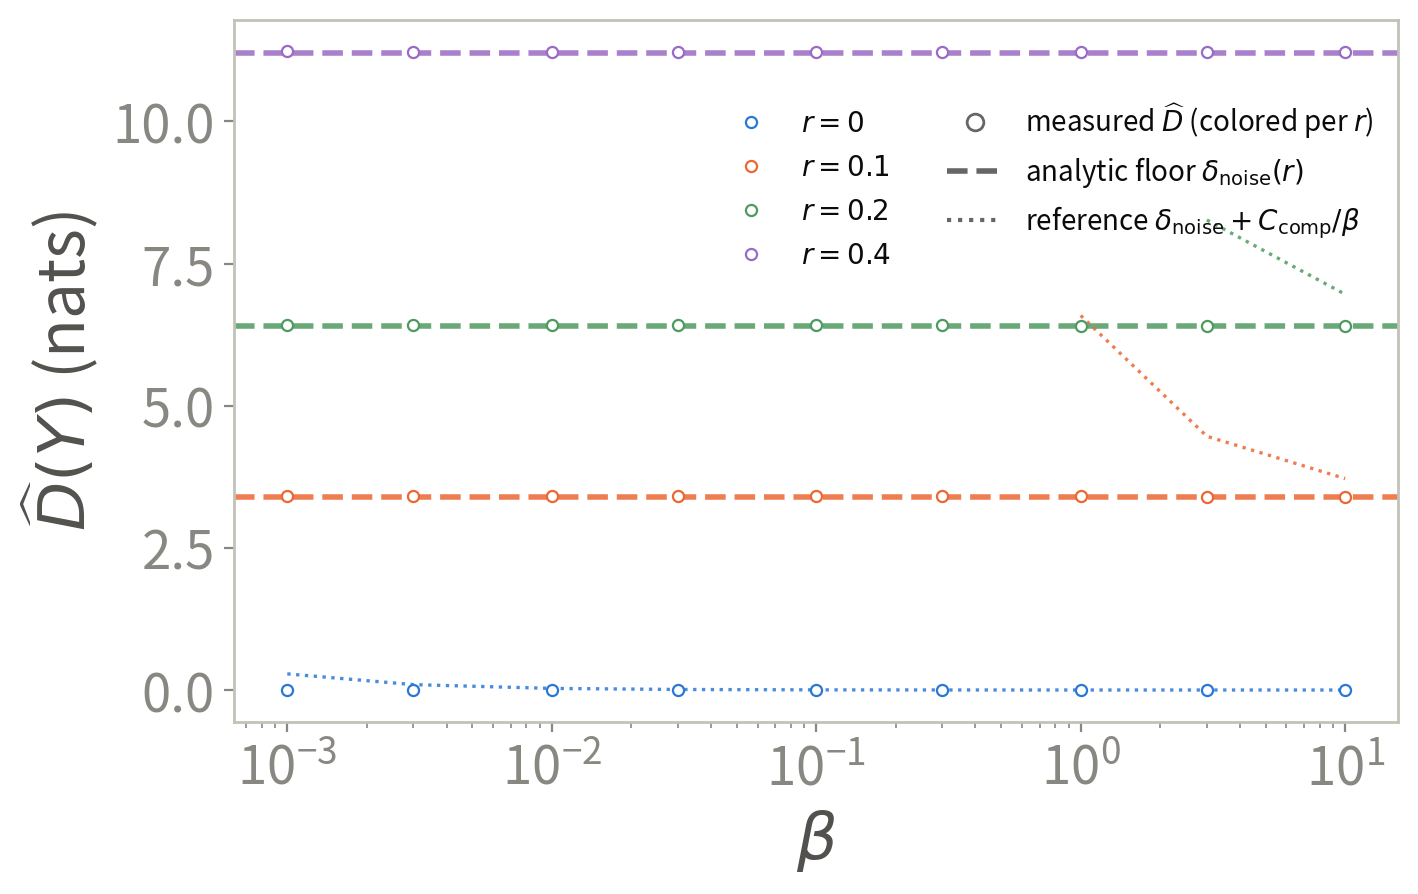
\includegraphics[width=0.32\linewidth]{figures/fig_noisy_appendix_i_varfixed.png}\hfill
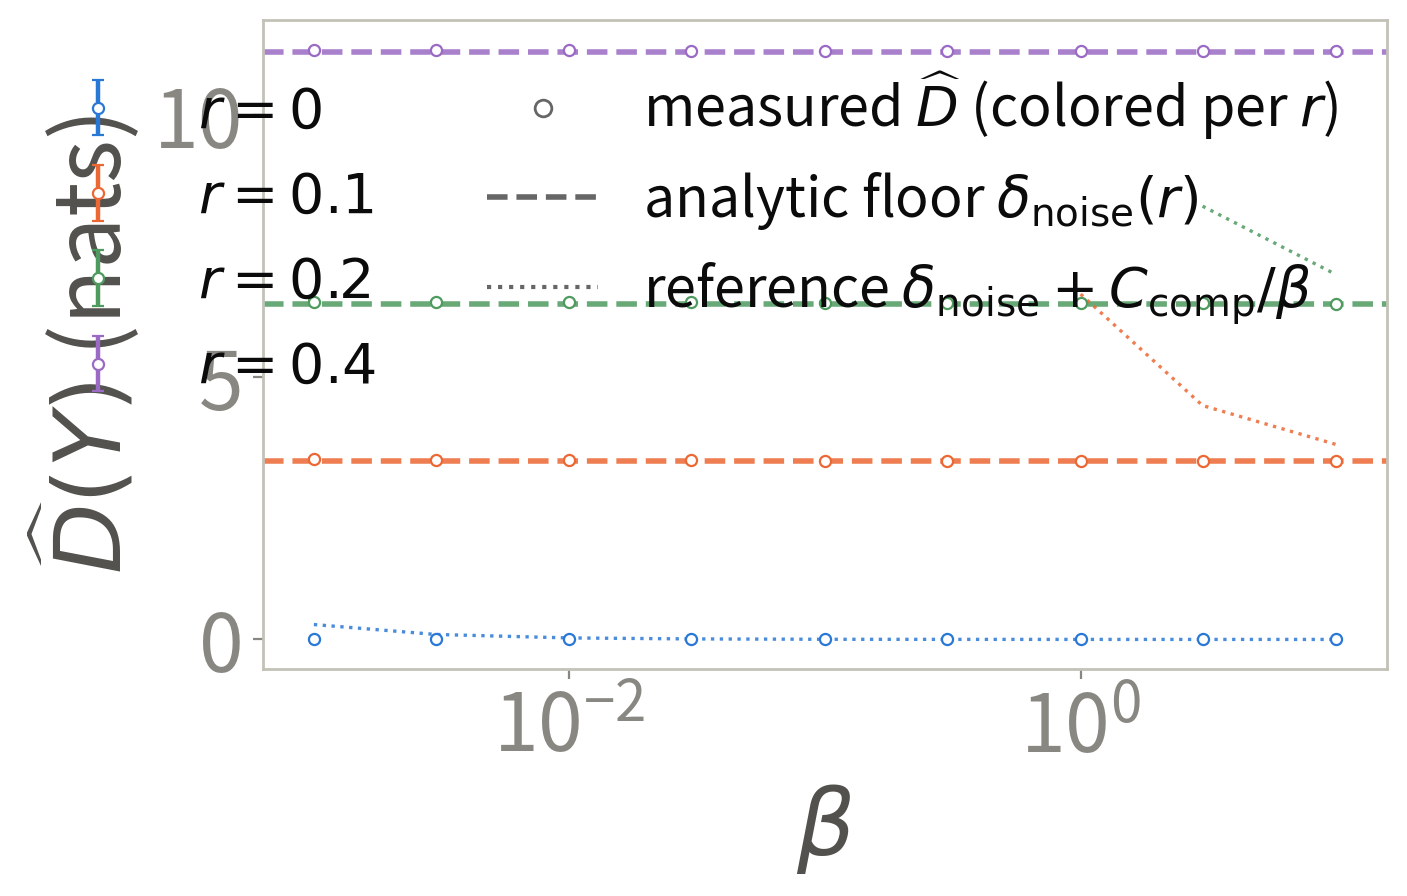
\includegraphics[width=0.32\linewidth]{figures/fig_noisy_appendix_ii_trainable.png}\hfill
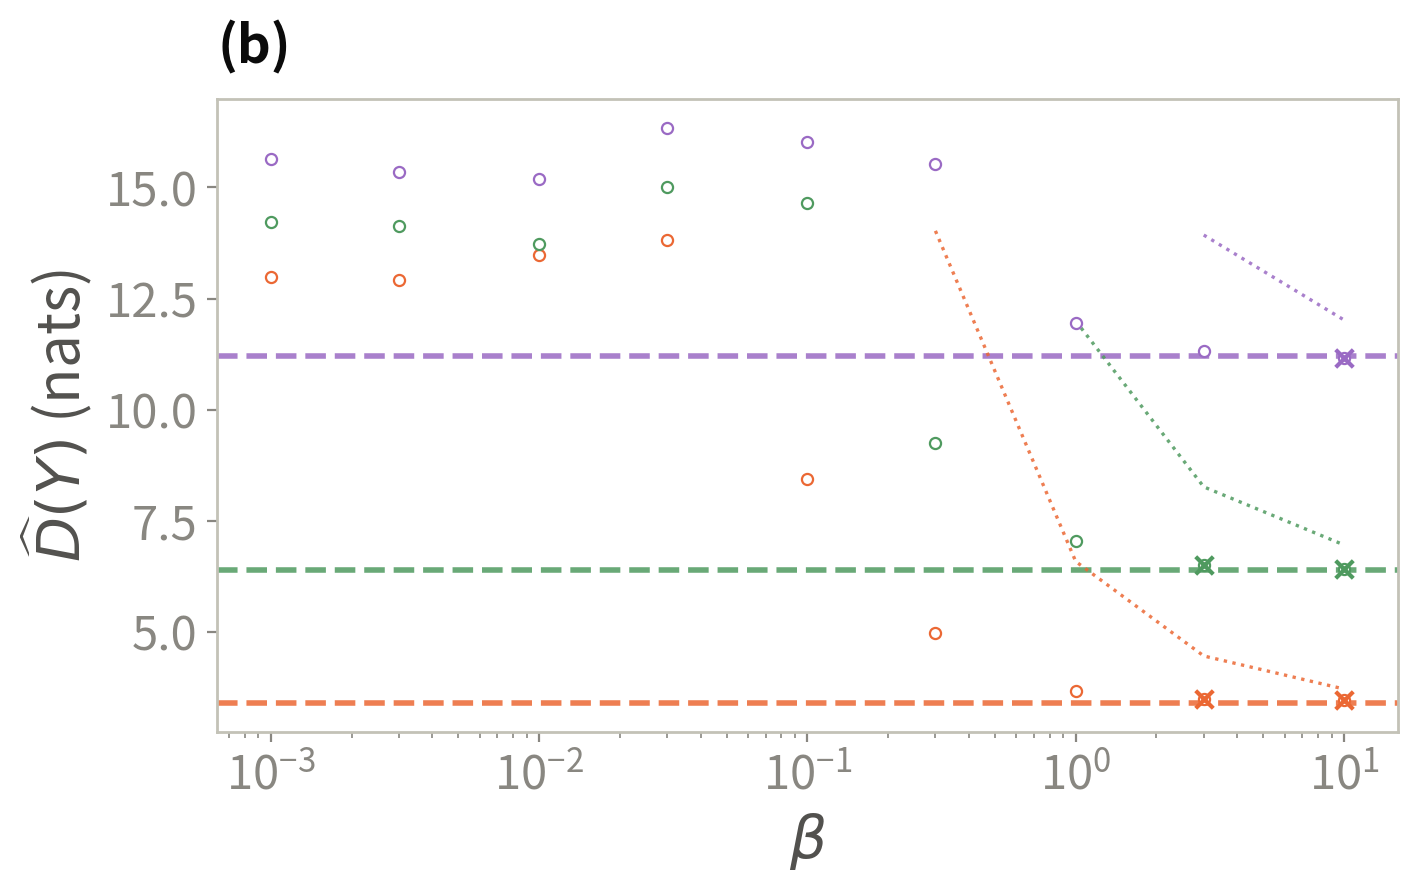
\includegraphics[width=0.32\linewidth]{figures/fig_noisy_appendix_iii_sampled.png}
\caption{Sensitivity analyses for the controlled label-ambiguity experiment.
(a) Posterior variance fixed to the prior variance. (b) Trainable stateless polar
frame. (c) Labels sampled rather than integrated with their exact population weights;
failed comparator-gate configurations are marked. Dashed lines denote the analytic
population ambiguity floors. Points are means and error bars are standard deviations
over five seeds.}
\label{fig:noisy-alignment-sensitivity}
\end{figure*}

\subsection{Direct mismatch definitions and separation diagnostics}
\label{app:direct-mismatch}

This section collects the diagnostic panels deferred from
Section~\ref{sec:direct-mismatch}: the decoupling scatter, the separation-bound and
slack readings, and the regression diagnostics, together with the finite-bin
definitions. All statistics are first computed within each seed and then aggregated
across the five seeds; class or bin pairs are not treated as independent
replicates. Every checkpoint in both requested grids is present, and no collapse or
variance-explosion point is removed.

The deferred classification panels complete the picture
(Fig.~\ref{fig:direct-mismatch-deferred}). The decoupling scatter (a) shows MC-10
accuracy staying within $82$--$86\%$ while $\widehat D$ spans three orders of
magnitude: mechanism and task metric are decoupled. Panel (b) shows the raw bound
rising toward the declared $\sqrt2a$ exactly where the mismatch corrections shrink,
so the slack narrows where the bound is informative; CEB's mismatch is plotted
descriptively, without a bound, since its reference has no declared $\Delta$. The
slack percentiles (c) stay non-negative at every reported point: the bound is
consistent but conservative.

\begin{figure*}[t]
\centering
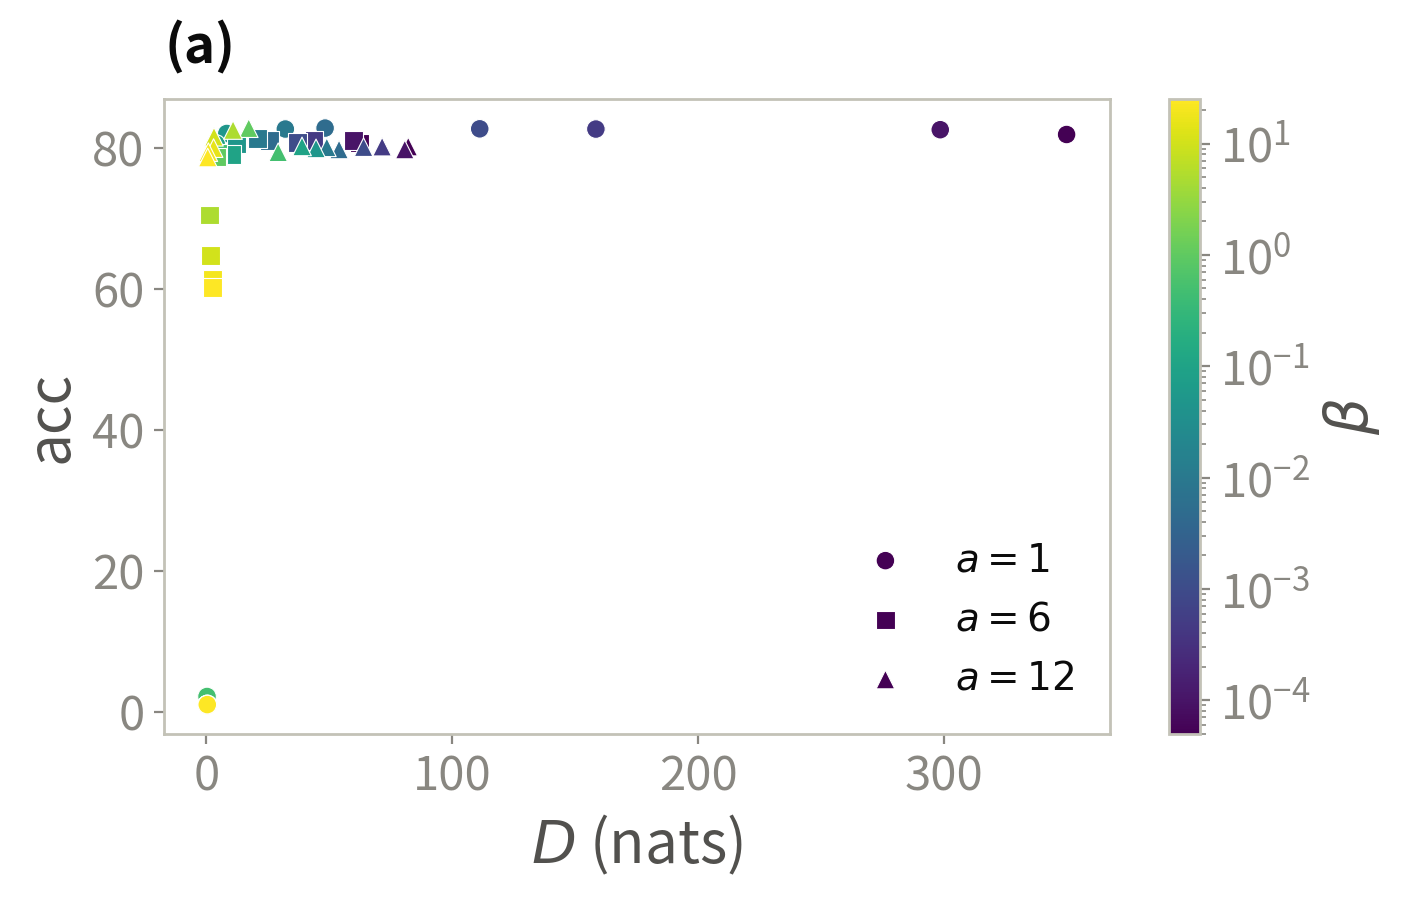
\includegraphics[width=0.24\linewidth]{figures/fig_mismatch_b_imagenet100_acc_vs_d.png}\hfill
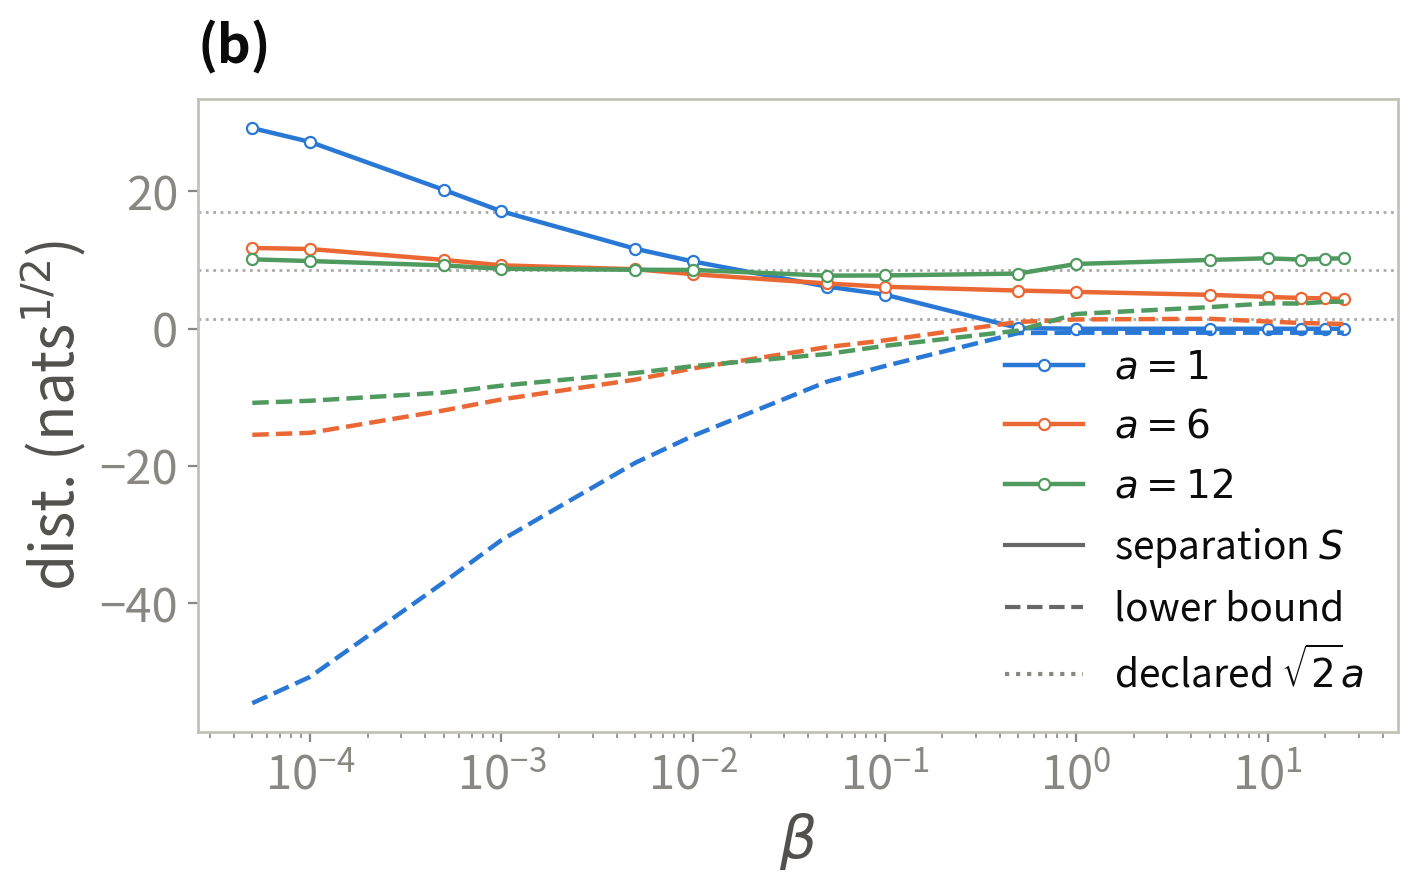
\includegraphics[width=0.24\linewidth]{figures/fig_mismatch_appendix_cls_i_separation_beta.png}\hfill
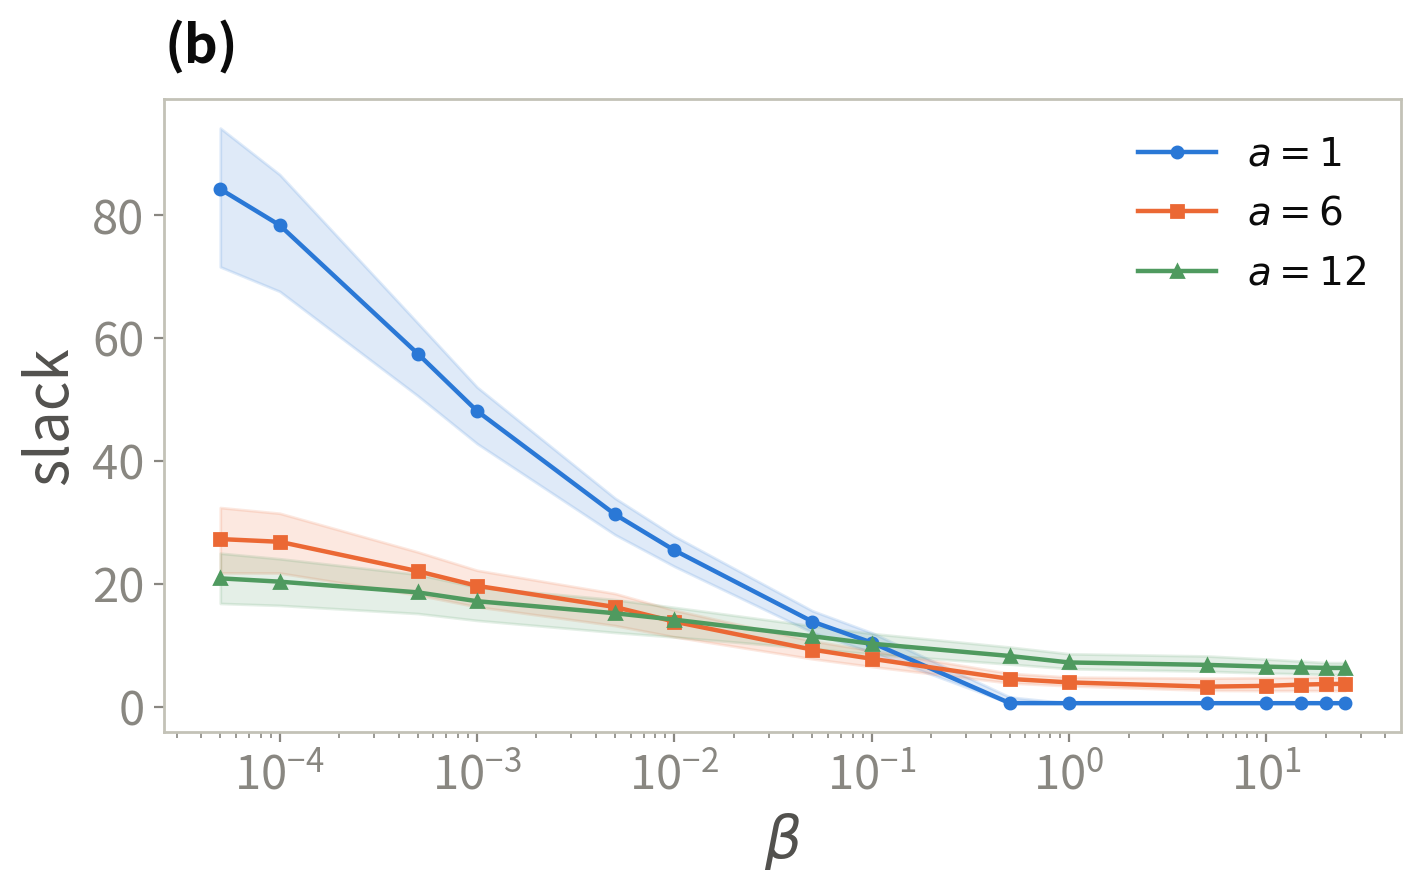
\includegraphics[width=0.24\linewidth]{figures/fig_mismatch_appendix_cls_iii_slack.png}\hfill
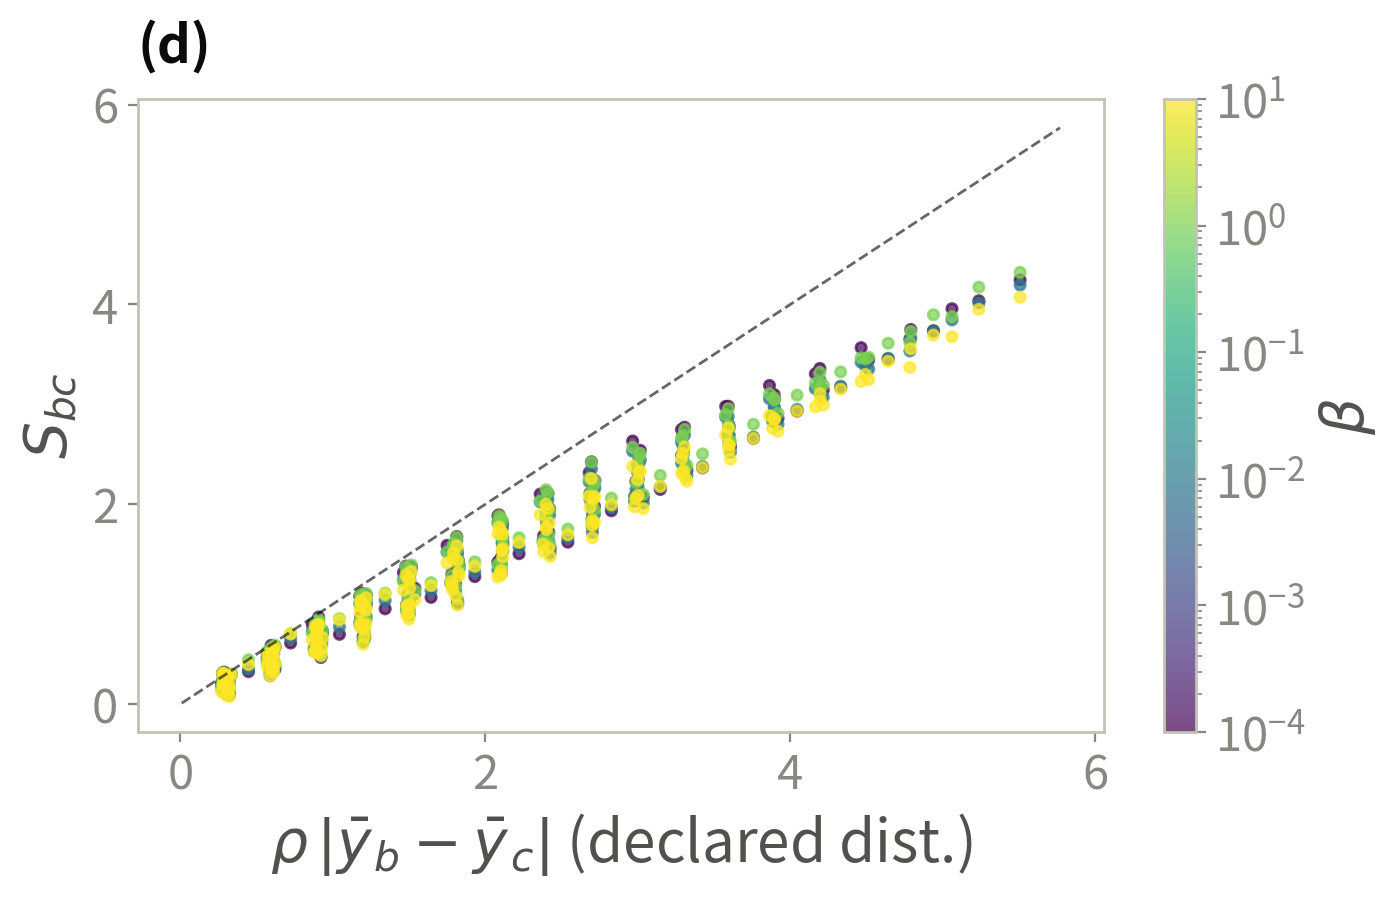
\includegraphics[width=0.24\linewidth]{figures/fig_mismatch_appendix_reg_binscatter.png}
\caption{Direct mismatch diagnostics deferred from the main text. (a) MC-10
accuracy against $\widehat D$ (color $=\beta$, marker $=a$). (b) Mean separation
(solid) and raw lower bound (dashed) against $\beta$; gray dotted: CEB,
descriptive. (c) Slack percentiles. (d) Cal.\ Housing bin-pair separation against
the declared prior distance at $\rho=6$ (color $=\beta$; identity line: exact
transfer). Means and standard deviations are over five seeds; no checkpoint is
omitted.}
\label{fig:direct-mismatch-deferred}
\end{figure*}

\paragraph{Regression.} We partition the standardized test labels into $20$
equal-width bins and merge any bin containing fewer than $30$ examples. Let
$\bar y_b$ be the mean label of bin $B_b$, $\widehat m_b$ its posterior center,
$\widehat D_b$ its average sample-to-own-anchor mismatch, and
$h_b:=\operatorname{diam}(B_b)$. The finite-bin lower bound is
\begin{equation}
\widehat{\mathrm{LB}}_{bc}
=\rho|\bar y_b-\bar y_c|
-\sqrt{2\widehat\tau^2_{\max}\widehat D_b}
-\sqrt{2\widehat\tau^2_{\max}\widehat D_c}
-\rho(h_b+h_c),
\label{eq:empirical-regression-separation-bound}
\end{equation}
where the last term is the quantization correction of
Remark~\ref{rem:pgib-binning}. On Housing with $\rho=6$, mismatch falls from
$0.264$ to $0.026$, the axial slope remains $0.73$--$0.77$, and the mismatch is
almost entirely axial (about $0.2$ against $0.004$ off-axis), while $R^2$ changes
only from $0.786$ to $0.767$ over the sweep: a tenfold mismatch reduction need not
imply a comparable task-metric gain. Figure~\ref{fig:direct-mismatch-deferred}d
plots the actual bin-center distances against the declared isometric distances at
$\rho=6$: the cloud hugs a line of slope $0.73$--$0.77$ below the identity line at
all four $\beta$ values, so the posterior follows the declared metric structure at
about three quarters of its scale, and the scale-transfer ratio is essentially
$\beta$-invariant. After the quantization correction, $43\%$ of bin pairs retain a
positive bound. Figure~\ref{fig:direct-mismatch-housing} shows the two regression
sweep panels: the mismatch--$\beta$ curves with their axial/off-axis decomposition
(the dotted off-axis contribution stays below $0.01$ nats, so the posterior lies
essentially on the declared axis), and the $R^2$-against-$\widehat D$ scatter whose
band stays within $0.75$--$0.79$ while $\widehat D$ spans orders of magnitude.

\begin{figure*}[t]
\centering
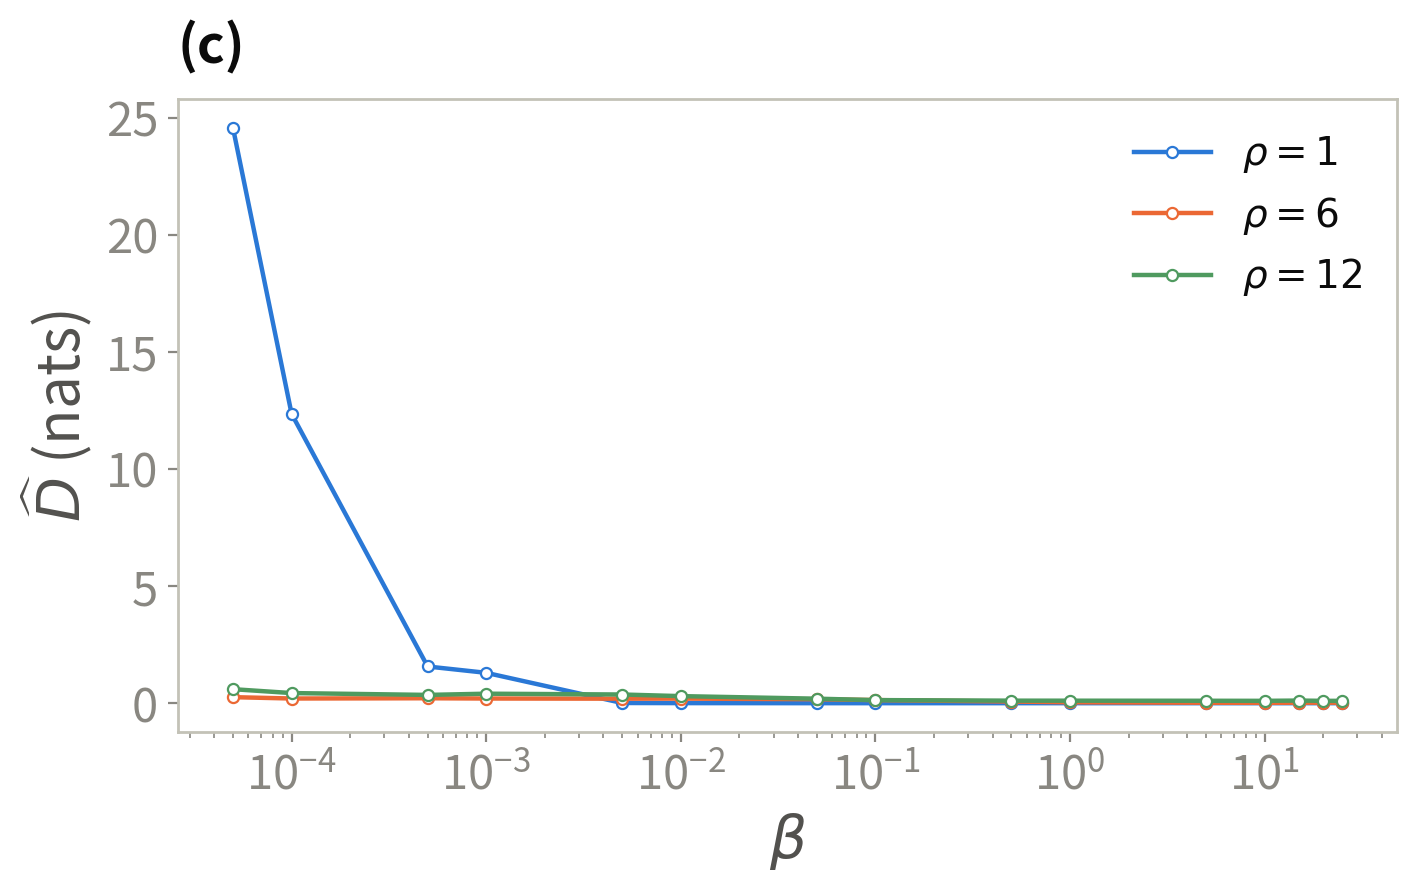
\includegraphics[width=0.48\linewidth]{figures/fig_mismatch_c_housing_d_beta.png}\hfill
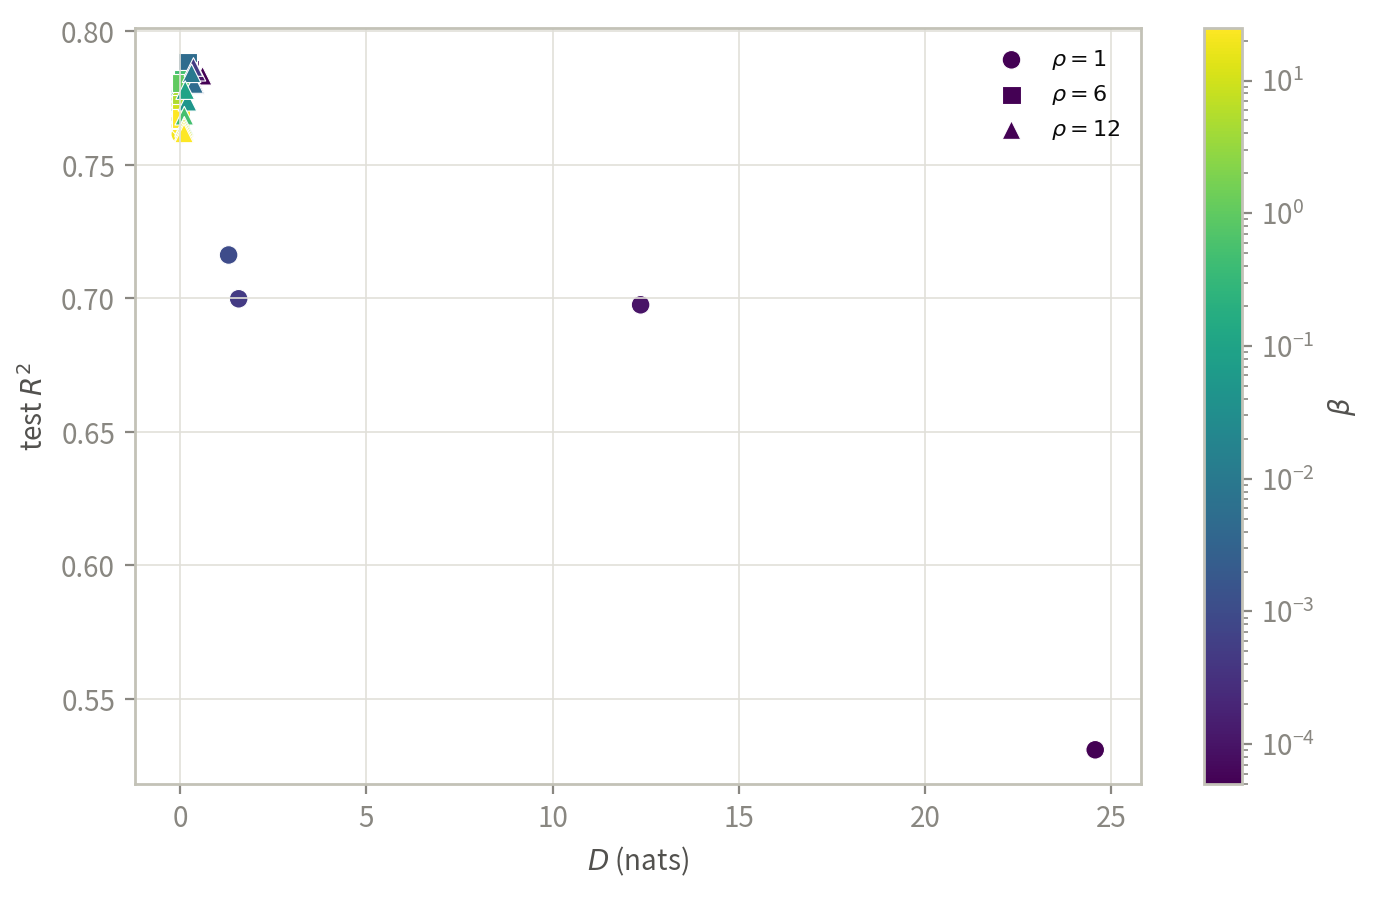
\includegraphics[width=0.48\linewidth]{figures/fig_mismatch_d_housing_r2_vs_d.png}
\caption{Cal.\ Housing mismatch sweep panels (deferred from the main text). (a)
Anchor mismatch $\widehat D$ against $\beta$, by isometric scale $\rho$, decomposed
into axial and off-axis contributions. (b) Test $R^2$ against $\widehat D$; color
denotes $\beta$ and marker shape $\rho$. Means and standard deviations are over five
seeds; no checkpoint is omitted.}
\label{fig:direct-mismatch-housing}
\end{figure*}

\paragraph{Normalization and variance extremes.} The empirical mismatch uses one
maximum conditional-reference variance per checkpoint, whereas the exact Gaussian KL
uses every sample's and coordinate's own variance. They therefore need not coincide:
averaged over the ImageNet-100 grid, $\widehat D=41.2$, the KL mean term is $46.5$,
and the KL variance term is $51.4$. On Housing, a small number of weak-compression,
large-$\rho$ variance explosions raise the across-grid mean KL variance term to
$2.8\times10^6$. These checkpoints remain in all plots. Because their
$\widehat\tau^2_{\max}$ is also large, the normalized $\widehat D$ can fall even as
the KL variance term grows; the unnormalized axial/off-axis components and total KL
are therefore reported alongside it.

\subsection{Main results with standard deviations}
\label{app:main-std}

Tables~\ref{tab:main_result_std_baselines} and~\ref{tab:main_result_std_variants}
report the same configurations as the main table with standard deviations over
runs, split by column groups for width (the baselines table includes NCBD and the
variants table includes AdaCap); bold and underline follow the same
mean-based rule as Table~\ref{tab:main_result}.

% 主结果表（带标准差）：由 paper/make_table.py 从 tune_results/*.html 自动生成，请勿手改。
% 因 8 方法列 × (均值±std) 超出页宽，按列拆为两张表：
% (a) baselines（Base/VIB/SVIB/NIB，tab:main_result_std_baselines）；
% (b) CEB/DVCCA 与 GPB/GPB-L（tab:main_result_std_variants，竖线分隔同主表）。
% 每表含全部 12 行；分类 Acc（%）、回归 R²，单元格为均值±std；
% 加粗/下划线按该行全部 8 列的均值判定（与 main_result.tex 一致）；
% 表尾排名行省略（与主表重复）。
\begin{table*}[t]
\centering
\caption{Test accuracy (\%) and test $R^2$ with standard deviations over runs: the plain backbone and the variational baselines; same configurations as Table~\ref{tab:main_result}.}
\label{tab:main_result_std_baselines}
\small
{
\setlength{\tabcolsep}{2pt}
\begin{tabular}{llcccc}
\hline
Dataset & Backbone & Base & VIB & SVIB & NIB \\
\hline
MNIST & MLP & 98.33$\pm$0.12 & 98.28$\pm$0.11 & 98.15$\pm$0.13 & 98.27$\pm$0.07 \\
MNIST & CNN & 99.13$\pm$0.05 & 99.28$\pm$0.09 & 99.23$\pm$0.03 & 99.22$\pm$0.06 \\
ImageNet-100 & MLP & 83.12$\pm$0.14 & 82.84$\pm$0.44 & 83.02$\pm$0.37 & 82.35$\pm$0.27 \\
ImageNet-100 & CNN & 83.40$\pm$0.13 & 82.94$\pm$0.37 & 83.11$\pm$0.86 & 82.91$\pm$0.35 \\
Cora & GCN & 87.68$\pm$0.46 & 86.83$\pm$0.28 & 86.46$\pm$1.87 & 86.35$\pm$0.68 \\
IMDb & RNN & 84.85$\pm$0.68 & 85.50$\pm$0.91 & 85.99$\pm$0.30 & 86.14$\pm$0.92 \\
AG News & RNN & \textbf{92.94$\pm$0.15} & 92.72$\pm$0.17 & 92.86$\pm$0.21 & 92.91$\pm$0.22 \\
\hline\hline
Cal. Housing & MLP & 0.7618$\pm$0.0238 & \underline{0.7901$\pm$0.0049} & 0.7897$\pm$0.0058 & 0.7862$\pm$0.0035 \\
STS-B & RNN & \textbf{0.2899$\pm$0.0113} & 0.2719$\pm$0.0164 & 0.2697$\pm$0.0202 & 0.2417$\pm$0.0221 \\
ZINC & GCN & \textbf{0.6348$\pm$0.0044} & 0.6339$\pm$0.0033 & 0.6325$\pm$0.0026 & 0.6178$\pm$0.0099 \\
AgeDB & MLP & 0.2180$\pm$0.0409 & 0.3173$\pm$0.0101 & \underline{0.3385$\pm$0.0286} & 0.2710$\pm$0.0235 \\
AgeDB & CNN & 0.3914$\pm$0.0194 & 0.3342$\pm$0.1894 & 0.3323$\pm$0.1870 & 0.3337$\pm$0.1889 \\
\hline
\end{tabular}
}
\end{table*}
\par\smallskip
\begin{table*}[t]
\centering
\caption{Test accuracy (\%) and test $R^2$ with standard deviations over runs: CEB, DVCCA, and our method; same configurations as Table~\ref{tab:main_result}. GPB and GPB-L are separated from the references by the vertical rule.}
\label{tab:main_result_std_variants}
\small
{
\setlength{\tabcolsep}{2pt}
\begin{tabular}{llcc|cc}
\hline
Dataset & Backbone & CEB & DVCCA & GPB & GPB-L \\
\hline
MNIST & MLP & \underline{98.43$\pm$0.08} & 98.24$\pm$0.17 & \textbf{98.54$\pm$0.09} & \underline{98.43$\pm$0.07} \\
MNIST & CNN & 99.30$\pm$0.05 & 99.29$\pm$0.10 & \textbf{99.32$\pm$0.05} & \underline{99.31$\pm$0.05} \\
ImageNet-100 & MLP & 82.77$\pm$0.22 & 82.99$\pm$0.43 & \textbf{84.40$\pm$0.21} & \underline{84.01$\pm$0.23} \\
ImageNet-100 & CNN & 82.97$\pm$0.67 & 83.21$\pm$0.70 & \textbf{86.08$\pm$0.21} & \underline{84.88$\pm$0.80} \\
Cora & GCN & 86.27$\pm$0.38 & 86.90$\pm$0.94 & \textbf{88.12$\pm$0.55} & \underline{87.86$\pm$0.87} \\
IMDb & RNN & 85.55$\pm$0.73 & 85.69$\pm$0.23 & \underline{86.84$\pm$0.57} & \textbf{86.99$\pm$0.35} \\
AG News & RNN & 92.83$\pm$0.11 & 92.78$\pm$0.15 & 92.87$\pm$0.12 & \underline{92.92$\pm$0.14} \\
\hline\hline
Cal. Housing & MLP & 0.7894$\pm$0.0018 & 0.7878$\pm$0.0048 & 0.7895$\pm$0.0051 & \textbf{0.7914$\pm$0.0034} \\
STS-B & RNN & 0.2668$\pm$0.0127 & 0.2713$\pm$0.0218 & \underline{0.2762$\pm$0.0152} & 0.2755$\pm$0.0134 \\
ZINC & GCN & 0.6257$\pm$0.0044 & 0.6294$\pm$0.0026 & \underline{0.6344$\pm$0.0031} & 0.6323$\pm$0.0016 \\
AgeDB & MLP & 0.3317$\pm$0.0251 & 0.3180$\pm$0.0228 & \textbf{0.3536$\pm$0.0076} & 0.3320$\pm$0.0080 \\
AgeDB & CNN & 0.3882$\pm$0.0275 & 0.3205$\pm$0.1811 & \textbf{0.4700$\pm$0.0072} & \underline{0.4388$\pm$0.0220} \\
\hline
\end{tabular}
}
\end{table*}
\par\smallskip


\subsection{Paired-difference confidence intervals}
\label{app:main-ci}

Tables~\ref{tab:main_result_ci_baselines}--\ref{tab:main_result_ci_external}
report, for each setting, the paired difference of GPB over every baseline
(GPB minus baseline) with a bootstrap $95\%$ confidence interval: the differences
are paired across the shared seeds, the interval is the percentile interval of
$B = 10{,}000$ resamples of the per-run differences (fixed seed, reproducible), and
the non-inferiority margin is $\delta = 0.2$ percentage points of accuracy or
$\delta = 0.005$ in $R^2$. Bold marks a lower bound above zero (significant
advantage) and $^{\dagger}$ a lower bound within the margin (tied); the best
configuration per method is the same as in the main table. The last table covers
the external non-IB baselines, NCBD on the classification settings and AdaCap on
the regression settings; the only interval lying entirely below zero is AdaCap on
ZINC ($-0.043$ $R^2$).

% 主结果差值 CI 表：由 paper/make_table.py 从 tune_results 自动生成，请勿手改。
% 行 = 12 个 setting；单元格 = GPB − baseline 的配对差值 [bootstrap 95% CI]
%（分类百分点、回归 R²）；加粗 = CI 下限 > 0（显著更优）、† = CI 下限 > −δ
%（非劣界 δ=0.2 百分点 / 0.005）记 tied；
% 同 seed 配对（run 顺序即 seed 0..N−1），bootstrap B=10000（固定 seed 0，百分位法）。
% 因 7 个差值列超页宽，按列拆两张表（baselines / ceb+dvcca+OPB-L）；表尾一行统计各列 */† 次数。
\begin{table*}[t]
\centering
\caption{Paired-difference 95\% confidence intervals of GPB over the plain backbone and VIB (GPB minus baseline, per setting; classification in percentage points, regression in $R^2$). Bold: lower CI bound above zero; $^{\dagger}$: lower bound within the non-inferiority margin $\delta$ (tied).}
\label{tab:main_result_ci_baselines}
\small
{
\setlength{\tabcolsep}{1pt}
\begin{tabular}{llcc}
\hline
Dataset & Backbone & Base & VIB \\
\hline
MNIST & MLP & \textbf{+0.2 [+0.2, +0.3]} & \textbf{+0.3 [+0.2, +0.3]} \\
MNIST & CNN & \textbf{+0.2 [+0.2, +0.2]} & +0.0 [-0.0, +0.1]$^{\dagger}$ \\
ImageNet-100 & MLP & \textbf{+1.3 [+1.2, +1.4]} & \textbf{+1.6 [+1.4, +1.9]} \\
ImageNet-100 & CNN & \textbf{+2.7 [+2.5, +2.9]} & \textbf{+3.1 [+3.0, +3.4]} \\
Cora & GCN & +0.4 [-0.1, +1.1]$^{\dagger}$ & \textbf{+1.3 [+0.7, +1.7]} \\
IMDb & RNN & \textbf{+2.0 [+1.2, +2.7]} & \textbf{+1.3 [+0.6, +2.3]} \\
AG News & RNN & -0.1 [-0.2, +0.0]$^{\dagger}$ & \textbf{+0.2 [+0.1, +0.2]} \\
\hline\hline
Cal. Housing & MLP & \textbf{+0.028 [+0.008, +0.048]} & -0.001 [-0.005, +0.003]$^{\dagger}$ \\
STS-B & RNN & -0.014 [-0.022, -0.006] & +0.004 [-0.017, +0.022] \\
ZINC & GCN & -0.000 [-0.003, +0.002]$^{\dagger}$ & +0.001 [-0.004, +0.004]$^{\dagger}$ \\
AgeDB & MLP & \textbf{+0.136 [+0.104, +0.167]} & \textbf{+0.036 [+0.026, +0.046]} \\
AgeDB & CNN & \textbf{+0.079 [+0.066, +0.091]} & \textbf{+0.136 [+0.043, +0.302]} \\
\hline
 &  & 8*/3† & 8*/3† \\
\hline
\end{tabular}
}
\end{table*}
\par\smallskip
\begin{table*}[t]
\centering
\caption{Paired-difference 95\% confidence intervals of GPB over SVIB and NIB (GPB minus baseline, per setting; classification in percentage points, regression in $R^2$). Bold/† as in the baselines table.}
\label{tab:main_result_ci_svib_nib}
\small
{
\setlength{\tabcolsep}{1pt}
\begin{tabular}{llcc}
\hline
Dataset & Backbone & SVIB & NIB \\
\hline
MNIST & MLP & \textbf{+0.4 [+0.3, +0.5]} & \textbf{+0.3 [+0.2, +0.3]} \\
MNIST & CNN & \textbf{+0.1 [+0.1, +0.1]} & \textbf{+0.1 [+0.1, +0.2]} \\
ImageNet-100 & MLP & \textbf{+1.4 [+1.1, +1.7]} & \textbf{+2.1 [+1.8, +2.2]} \\
ImageNet-100 & CNN & \textbf{+3.0 [+2.4, +3.9]} & \textbf{+3.2 [+2.9, +3.5]} \\
Cora & GCN & \textbf{+1.7 [+0.2, +3.4]} & \textbf{+1.8 [+1.1, +2.4]} \\
IMDb & RNN & \textbf{+0.8 [+0.2, +1.4]} & \textbf{+0.7 [+0.2, +1.2]} \\
AG News & RNN & +0.0 [-0.1, +0.1]$^{\dagger}$ & -0.0 [-0.2, +0.1]$^{\dagger}$ \\
\hline\hline
Cal. Housing & MLP & -0.000 [-0.006, +0.004] & +0.003 [-0.001, +0.009]$^{\dagger}$ \\
STS-B & RNN & +0.006 [-0.021, +0.028] & \textbf{+0.035 [+0.011, +0.058]} \\
ZINC & GCN & +0.002 [-0.001, +0.004]$^{\dagger}$ & \textbf{+0.017 [+0.010, +0.026]} \\
AgeDB & MLP & +0.015 [-0.010, +0.041] & \textbf{+0.083 [+0.062, +0.100]} \\
AgeDB & CNN & \textbf{+0.138 [+0.045, +0.303]} & \textbf{+0.136 [+0.040, +0.302]} \\
\hline
 &  & 7*/2† & 10*/2† \\
\hline
\end{tabular}
}
\end{table*}
\par\smallskip
\begin{table*}[t]
\centering
\caption{Paired-difference 95\% confidence intervals of GPB over CEB, DVCCA, and the free-head ablation OPB-L (GPB minus baseline, per setting; classification in percentage points, regression in $R^2$). Bold/† as in the baselines table.}
\label{tab:main_result_ci_variants}
\small
{
\setlength{\tabcolsep}{1pt}
\begin{tabular}{llccc}
\hline
Dataset & Backbone & CEB & DVCCA & OPB-L \\
\hline
MNIST & MLP & \textbf{+0.1 [+0.0, +0.2]} & \textbf{+0.3 [+0.2, +0.4]} & \textbf{+0.1 [+0.0, +0.2]} \\
MNIST & CNN & +0.0 [-0.0, +0.1]$^{\dagger}$ & +0.0 [-0.1, +0.1]$^{\dagger}$ & +0.0 [-0.0, +0.1]$^{\dagger}$ \\
ImageNet-100 & MLP & \textbf{+1.6 [+1.5, +1.7]} & \textbf{+1.4 [+1.1, +1.7]} & \textbf{+0.4 [+0.2, +0.5]} \\
ImageNet-100 & CNN & \textbf{+3.1 [+2.4, +3.7]} & \textbf{+2.9 [+2.4, +3.5]} & \textbf{+1.2 [+0.5, +1.9]} \\
Cora & GCN & \textbf{+1.8 [+1.5, +2.3]} & \textbf{+1.2 [+0.4, +1.9]} & +0.3 [-0.5, +1.3] \\
IMDb & RNN & \textbf{+1.3 [+0.3, +2.1]} & \textbf{+1.1 [+0.8, +1.5]} & -0.2 [-0.6, +0.5] \\
AG News & RNN & +0.0 [-0.1, +0.2]$^{\dagger}$ & +0.1 [-0.0, +0.2]$^{\dagger}$ & -0.0 [-0.2, +0.1]$^{\dagger}$ \\
\hline\hline
Cal. Housing & MLP & +0.000 [-0.003, +0.004]$^{\dagger}$ & +0.002 [-0.005, +0.009] & -0.002 [-0.005, +0.002] \\
STS-B & RNN & +0.009 [-0.009, +0.025] & +0.005 [-0.020, +0.026] & +0.001 [-0.019, +0.017] \\
ZINC & GCN & \textbf{+0.009 [+0.005, +0.011]} & \textbf{+0.005 [+0.002, +0.007]} & +0.002 [-0.001, +0.005]$^{\dagger}$ \\
AgeDB & MLP & \textbf{+0.022 [+0.006, +0.038]} & \textbf{+0.036 [+0.012, +0.057]} & \textbf{+0.022 [+0.019, +0.025]} \\
AgeDB & CNN & \textbf{+0.082 [+0.064, +0.099]} & \textbf{+0.149 [+0.065, +0.310]} & \textbf{+0.031 [+0.018, +0.046]} \\
\hline
 &  & 8*/3† & 8*/2† & 5*/3† \\
\hline
\end{tabular}
}
\end{table*}
\par\smallskip


\subsection{Information-plane panels for Cal.~Housing}
\label{app:info-plane-extra}

Figure~\ref{fig:info-plane-extra} completes panels (c)--(d) of
Fig.~\ref{fig:compression-main} in the main text with the regression setting, under
the same $\beta$ grid, axis
conventions, and five runs per point; here
$I(Y;Z)$ is the Gaussian approximation
$\tfrac12 \ln\bigl(\mathrm{Var}(y)/\mathrm{Var}(y-\hat y)\bigr)$, a heuristic
rather than a bound. On Cal.~Housing this approximation consistently reads
above the InfoNCE bound, so the certificate panel reflects the estimator gap
rather than the geometry; the information plane remains informative: CEB
compresses itself off the task ($R^2 = 0.49$ at $\beta = 0.1$, $0.18$ at
$\beta = 0.5$) while every EPB curve keeps $R^2 \ge 0.76$ flat out to
$\beta = 25$.

\begin{figure*}[t]
\centering
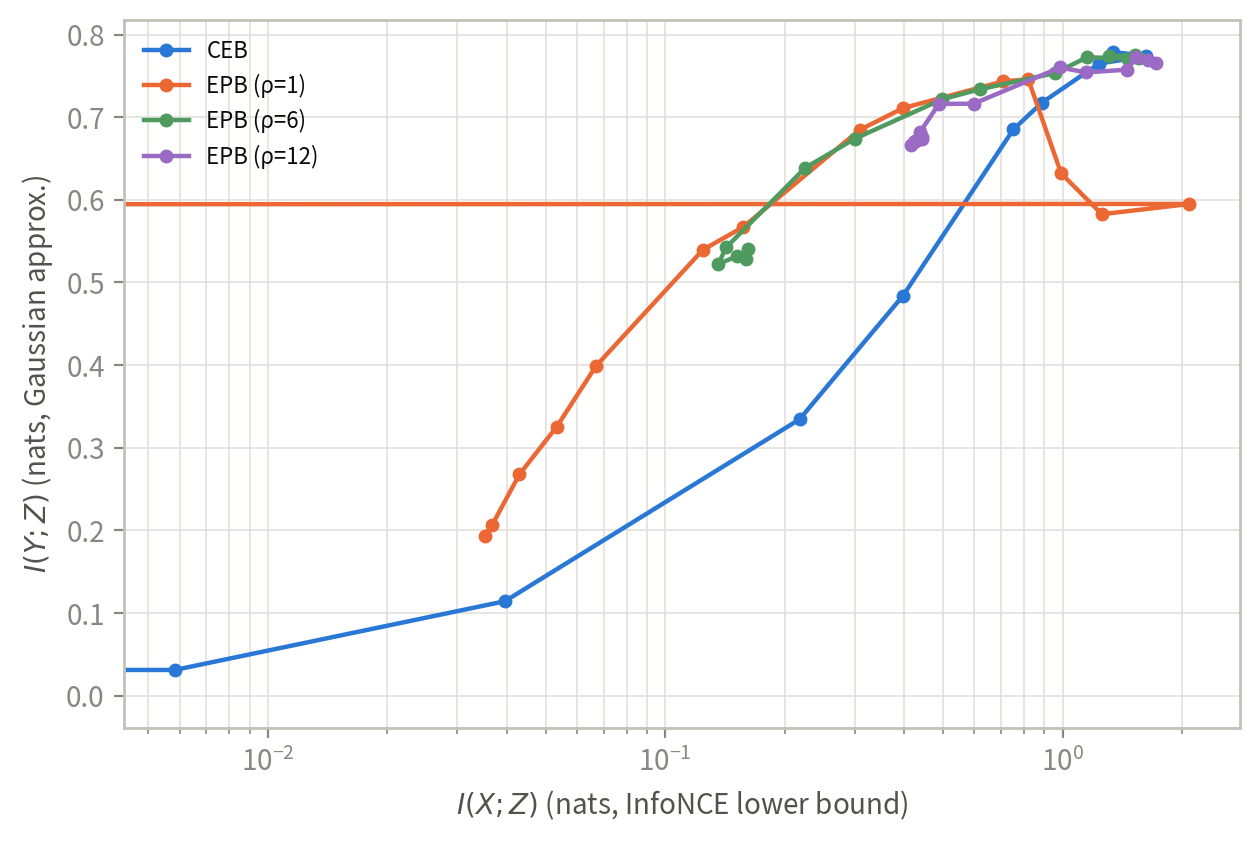
\includegraphics[width=0.48\linewidth]{figures/fig_info_plane_housing.png}\hfill
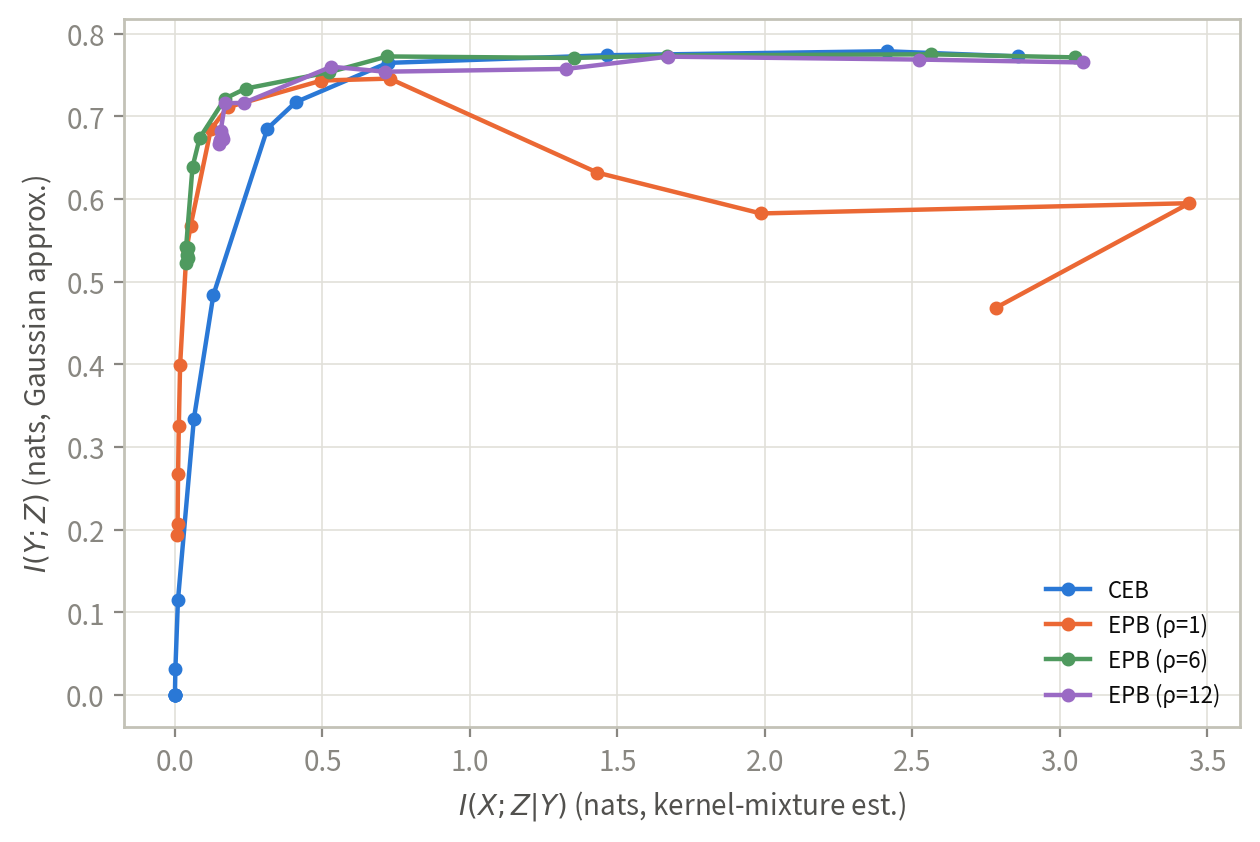
\includegraphics[width=0.48\linewidth]{figures/fig_certificate_plane_housing.png}
\caption{Information plane (a) and certificate plane (b) for Cal.~Housing,
companion panels to Fig.~\ref{fig:compression-main}(c,d): identical estimators,
$\beta$ grid (log $x$-scale in (a); linear where the estimated residual turns negative
in (b)), five runs per point, lines connect $\beta$ in ascending order. CEB
one curve per panel; EPB three ($\rho \in \{1, 6, 12\}$).}
\label{fig:info-plane-extra}
\end{figure*}

% =====================================================================
